\documentclass[12pt]{article}
\textwidth 15.5cm \oddsidemargin 0cm \topmargin -1cm \textheight 24cm \footskip 1.5cm
\usepackage{epsfig, amsmath,graphicx,psfrag,pstcol, float, listings, caption, array, verbatim}
\newenvironment{metaverbatim}{\verbatim}{\endverbatim}
\def\n{\noindent}
\def\u{\underline}
\def\hs{\hspace}
\newcommand{\thrfor}{.^{\displaystyle .} .}
\newcommand{\bvec}[1]{{\bf #1}}
\captionsetup{justification=centering, width=0.9\textwidth}

\newfloat{lstfloat}{htbp}{lop}
\floatname{lstfloat}{Listing}
\lstset{basicstyle = \footnotesize, breaklines = true}

\begin{document}
Appendix only

\appendix
\section{Test definition files}
\subsection{Binary adder}
\begin{lstfloat}[H]
\begin{lstlisting}[frame=single, caption={Definition file of a 2-bit binary adder}\label{lst:1}]
//This one is a 2-bit binary adder with combinational logic
DEVICES	AND A1 2,
	AND A2 2,
	XOR X1,
	XOR X2,
	XOR X3,
	SWITCH S0 1,
	SWITCH S1 1,
	SWITCH S2 1,
	SWITCH S3 1;
CONNECT	S0 => A1.I1,
	S2 => A1.I2,
	S1 => A2.I1,
	S3 => A2.I2,
	S0 => X1.I1,
	S2 => X1.I2,
	S1 => X2.I1,
	S3 => X2.I2,
	A1 => X3.I1,
	X2 => X3.I2;
MONITOR	X1,
	X3,
	A2;
\end{lstlisting}
\end{lstfloat}

\begin{figure}[H]
  \centering
  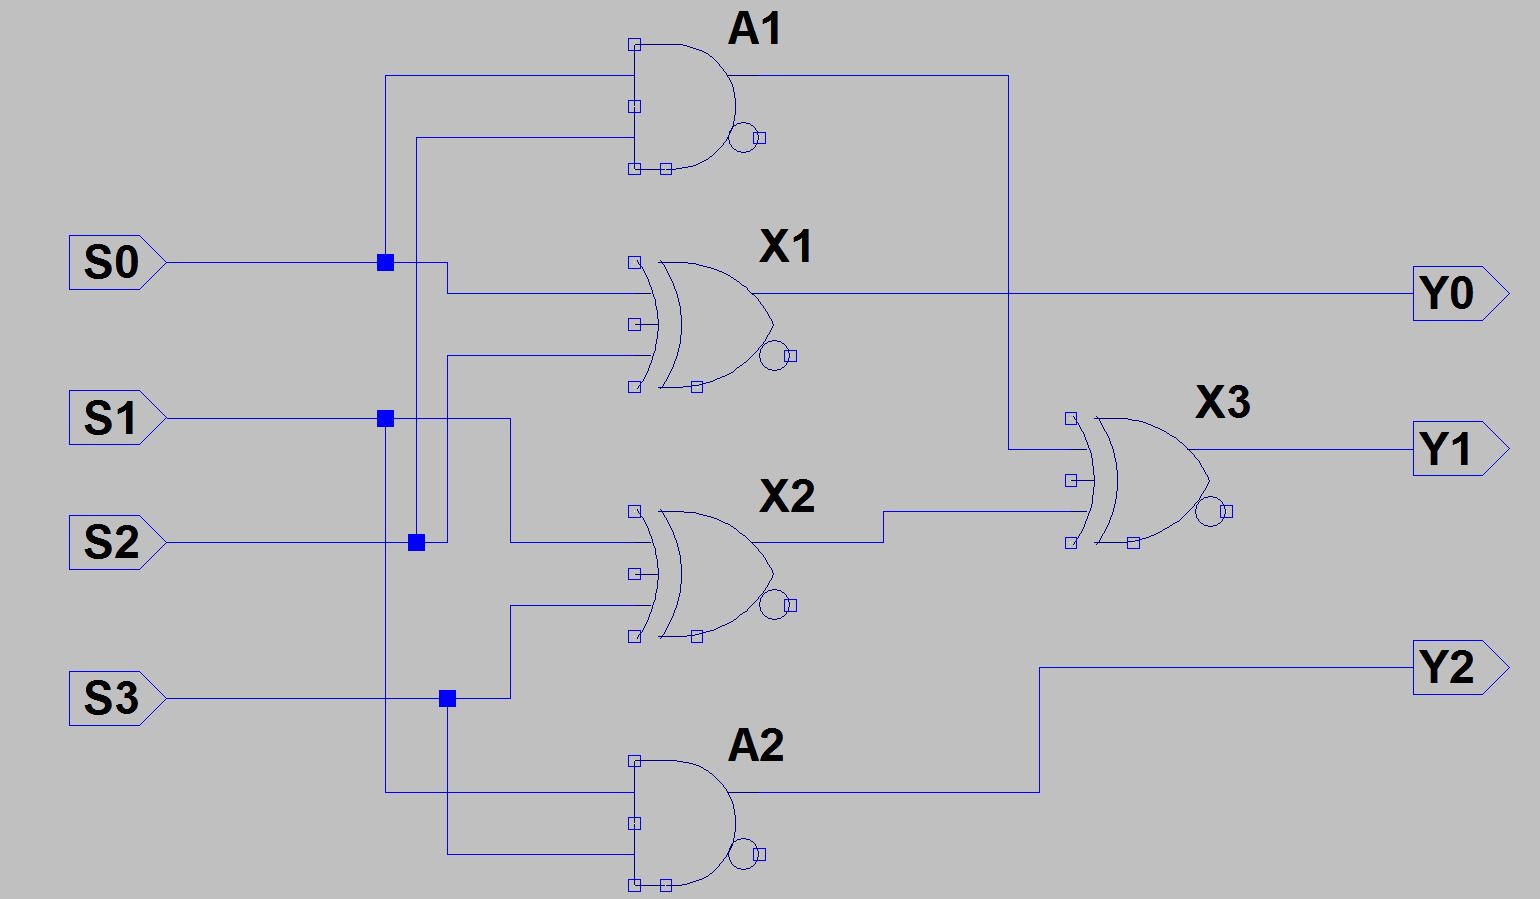
\includegraphics[width=0.9\linewidth]{figures/Test101.png}
  \captionsetup{width=.7\linewidth}
  \caption{File 1, Binary adder}
  \label{fig:1}
\end{figure}



\subsection{Vending machine}
\begin{lstlisting}[frame=single, caption={Vending machine circuit}\label{lst:2}]
//a vending machine where S1 and S2 indicate whether a 10p or 5p are inserted
DEVICES	SWITCH S1 1, 
	SWITCH S2 1,
	SWITCH S3 0,
	SWITCH S4 1,
	AND A1 2,
	AND A2 2,
	AND A3 2,
	AND A4 2,
	AND A5 2,
	AND A6 2,
	AND A7 2,
	AND A8 2,
	OR O1 4,
	OR O2 3,
	D_TYPE D1,
	D_TYPE D2,
	NAND N2 1,
	CLOCK CLK1 5,
	AND A9 2;
CONNECT	S2 => N2.I1,
	S1 => A1.I1,
	D1.QBAR => A1.I2,
	A1 => O1.I1,
	S1 => A2.I1,
	D2.QBAR => A2.I2,
	A2 => O1.I2,
	D1.Q => A3.I1,
	D2.QBAR => A3.I2,
	A3 => O1.I3,
	A3 => A8.I1,
	D1.QBAR => A4.I1,
	D2.Q => A4.I2,
	A4 => A6.I2,
	A4 => A7.I1,
	S2 => A5.I1,
	D2.QBAR => A5.I2,
	A5 => O2.I3,
	S2 => A6.I1,
	A6 => O1.I4,
	N2 => A7.I2,
	A7 => O2.I1,
	S1 => A8.I2,
	A8 => O2.I2,
	O1 => D1.DATA,
	O2 => D2.DATA,
	CLK1 => D1.CLK,
	CLK1 => D2.CLK,
	D1.Q => A9.I1,
	D2.Q => A9.I2,
	S3 => D1.SET,
	S3 => D2.SET,
	S4 => D1.CLEAR,
	S4 => D2.CLEAR;
MONITOR	A9,
	D1.Q,
	D2.Q;
\end{lstlisting}

\begin{figure}[H]
  \centering
  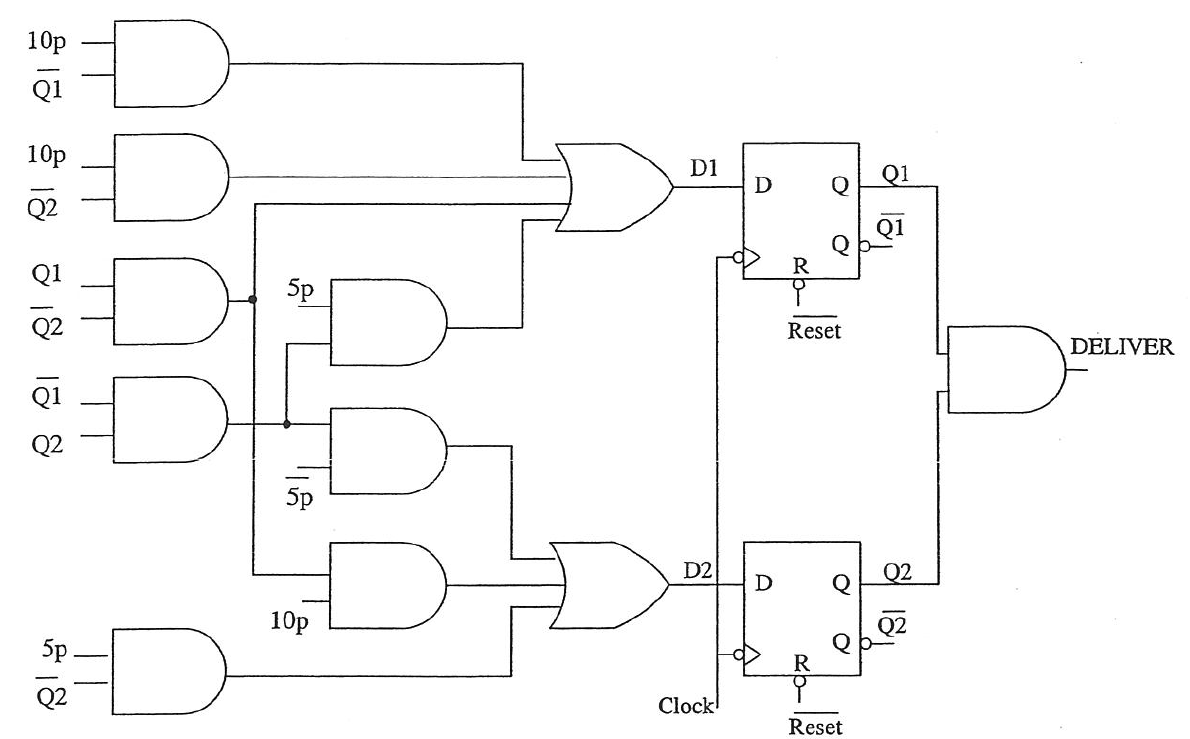
\includegraphics[width=0.9\linewidth]{figures/Test102.png}
  \captionsetup{width=.7\linewidth}
  \caption{File 2, Binary adder}
  \label{fig:2}
\end{figure}

\newpage
\subsection{Test 104}
\begin{lstlisting}[frame=single, caption={File 3}\label{lst:2}]
DEVICES	SWITCH S1 1,
	SWITCH S2 1,
	SWITCH S3 1,
	SWITCH S4 1,
	SWITCH S5 1,
	SWITCH S6 1,
	NAND A1 2,
	NAND A2 2,
	NAND A3 2,
	NAND A4 2,
	NAND A5 2,
	NAND A6 3,
	NAND A7 3,
	NAND A8 3,
	NOR N1 1,
	NOR N2 1,
	NOR N3 1;
CONNECT	S1 => A1.I1,
	S2 => A1.I2,
	A1 => A7.I2,
	A1 => A5.I1,
	S1 => N1.I1,
	N1 => A3.I1,
	S3 => A3.I2,
	A3 => A5.I2,
	A3 => A6.I2,
	S5 => A2.I1,
	S6 => A2.I2,
	A2 => A4.I1,
	S2 => N2.I1,
	N2 => A4.I2,
	A4 => A8.I3,
	S5 => N3.I1,
	N3 => A7.I1,
	A5 => A6.I1,
	S4 => A6.I3,
	S4 => A8.I2,
	A6 => A7.I3,
	A7 => A8.I1;
MONITOR A8;

\end{lstlisting}

\begin{figure}[H]
  \centering
  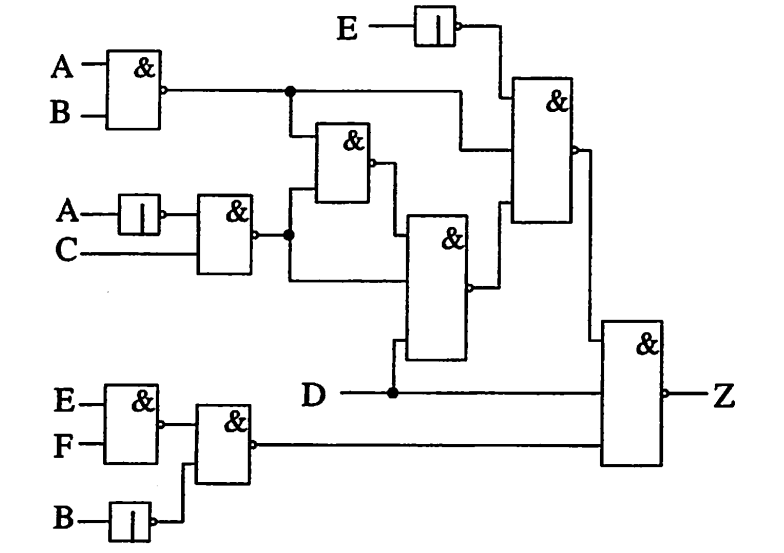
\includegraphics[width=0.9\linewidth]{figures/Test104.png}
  \captionsetup{width=.7\linewidth}
  \caption{File 3}
  \label{fig:3}
\end{figure}


\subsection{Incorrect test definition file}
\begin{lstlisting}[frame=single, caption={Faulty vending machine circuit}\label{lst:4}]
//a faulty vending machine where S1 and S2 indicate whether a 10p or 5p are inserted
DEVICES	SWITCH S1 1, 
	SWITCH S2 1,
	SWITCH SWITCH 1, //Unexpected Token: SWITCH cannot be device name
	SWITCH S4 3, //Semantic Error: Invalid switch
	AND A1, //Unexpected Token: Number of inputs not defined
	AND A2 2,
	AND A3 2,
	AND A4 22, //Semantic Error: Invalid gate
	AND A5 2,
	AND A6 2,
	AND A7 2,
	AND A8 2,
	OR jiangxueaihaozhe 4, //Warning: Name too long
	OR O2 3,
	D_TYPE O2, //Warning: Name conflict
	D_TYPE D2,
	NAND N2 1,
	CLOCK CLK1 5,
	AND u2he*2w 2; //Unexpected Token: Device name cannot contain *
CONNECT	S2 => N2.I1,
	S1 => A1.I1,
	D1.QBAR => A1.I2,
	A1 => O1.I1,
	S1 => A2.I1,
	D2.QBAR => A2.I2,
	A2 => O1.I2,
	D1.Q => A3.I1,
	D2.QBAR => A3.I2,
	A3.I2 => D1.Q, //Syntax Error: Not Output & Not Input
	A3 => O1.I3,
	A3 => A8.I1,
	A3.I1 => A4.I2, //Syntax Error: Not Output
	D1.QBAR => A4.I1,
	D2.Q => A4.I2,
	A4 => A6.I2,
	A4 => A7.I1,
	S2 => A5.I1,
	D2.QBAR => A5.I2,
	A4 => A5.I3, //Semantic Error: Undefined pin
	A5 => O2.I3,
	S2 => A6.I1,
	A6 => O1.I4,
	N2 => A7.I2,
	A7 => O2.I1,
	S1 => A8.I2,
	A8 => O2.I2,
	O1 => D1.DATA,
	O2 => D2.DATA,
	CLK1 => D1.CLK,
	CLK1 => D2.CLK //Unexpected Token: Missing a stop symbol
	D1.Q => A9.I1,
	D2.Q => A9.I2,
	S3 => D1.SET,
	S3 => D2.SET,
	S4 => D1.CLEAR,
	D1.QBAR => D2.Q, //Syntax Error: Not Input
	S4 => D2.CLEAR;
// Semantic Error: Floating Input
MONITOR	A9,
	D1.Q,
	D3.Q, //Semantic Error: Undefined device
	D2.Q;
\end{lstlisting}

\begin{lstlisting}[frame=single, caption={Error messages generated by the logic simulator}\label{lst:5}]
Expect Name Symbol
***Unxpected Token
	SWITCH SWITCH 1, 
	       ^
***Error: Invalid Switch
	SWITCH S4 3, 
	          ^
Expect a Number
***Unxpected Token
	AND A1, 
	      ^
***Error: Invalid Gate
	AND A4 22, 
	       ^
***Warning: Name Too Long
	OR jiangxueaihaozhe 4, 
	   ^
***Warning: Name Conflict
	D_TYPE O2, 
	       ^
Expect Name Symbol
***Unxpected Token
	AND u2he*2w 2; 
	    ^
***Error: Undefined Device
	S1 => A1.I1,
	      ^
***Error: Undefined Device
	D1.QBAR => A1.I2,
	^
***Error: Undefined Device
	D1.QBAR => A1.I2,
	           ^
***Error: Undefined Device
	A1 => O1.I1,
	^
***Error: Undefined Device
	A1 => O1.I1,
	      ^
***Error: Undefined Device
	A2 => O1.I2,
	      ^
***Error: Undefined Device
	D1.Q => A3.I1,
	^
***Error: Not an Output Pin
	A3.I2 => D1.Q, 
	^
***Error: Undefined Device
	A3.I2 => D1.Q, 
	         ^
***Error: Undefined Device
	A3 => O1.I3,
	      ^
***Error: Not an Output Pin
	A3.I1 => A4.I2, 
	^
***Error: Undefined Device
	A3.I1 => A4.I2, 
	         ^
***Error: Undefined Device
	D1.QBAR => A4.I1,
	^
***Error: Undefined Device
	D1.QBAR => A4.I1,
	           ^
***Error: Undefined Device
	D2.Q => A4.I2,
	        ^
***Error: Undefined Device
	A4 => A6.I2,
	^
***Error: Undefined Device
	A4 => A7.I1,
	^
***Error: Undefined Device
	A4 => A5.I3, 
	^
***Error: Undefined Pin
	A5 => O2.I3,
	      ^
***Error: Undefined Device
	A6 => O1.I4,
	      ^
***Error: Undefined Pin
	A7 => O2.I1,
	      ^
***Error: Undefined Pin
	A8 => O2.I2,
	      ^
***Error: Undefined Device
	O1 => D1.DATA,
	^
***Error: Undefined Device
	O1 => D1.DATA,
	      ^
***Error: Undefined Pin
	O2 => D2.DATA,
	^
***Error: Undefined Device
	CLK1 => D1.CLK,
	        ^
Expect Stop Symbol
***Unxpected Token
	D1.Q => A9.I1,
	^
***Error: Undefined Device
	D2.Q => A9.I2,
	        ^
***Error: Undefined Device
	S3 => D1.SET,
	^
***Error: Undefined Device
	S3 => D1.SET,
	      ^
***Error: Undefined Device
	S3 => D2.SET,
	^
***Error: Undefined Device
	S4 => D1.CLEAR,
	^
***Error: Undefined Device
	S4 => D1.CLEAR,
	      ^
***Error: Undefined Device
	D1.QBAR => D2.Q, 
	^
***Error: Not an Input Pin
	D1.QBAR => D2.Q, 
	           ^
***Error: Undefined Device
	S4 => D2.CLEAR;
	^
Unconnected Input : D2.CLEAR
Unconnected Input : D2.SET
Unconnected Input : D2.DATA
Unconnected Input : O2.CLEAR
Unconnected Input : O2.SET
Unconnected Input : O2.CLK
Unconnected Input : O2.DATA
Unconnected Input : O2.I3
Unconnected Input : O2.I2
Unconnected Input : O2.I1
Unconnected Input : jiangxue.I4
Unconnected Input : jiangxue.I3
Unconnected Input : jiangxue.I2
Unconnected Input : jiangxue.I1
Unconnected Input : A7.I1
Unconnected Input : A6.I2
Unconnected Input : A3.I1
***Error: Floating Input
MONITOR	A9,
^
***Error: Undefined Device
MONITOR	A9,
       	^
***Error: Undefined Device
	D1.Q,
	^
***Error: Undefined Device
	D3.Q, 
	^
Total Syntax Error Count: 7
Total Semantics Error Count: 38
Total Warning Count: 2

\end{lstlisting}

\begin{lstlisting}[frame=single, caption={Internally stored data}\label{lst:6}]
Monitored Outputs: 
29
Not Monitored Outputs: 
-29
-28
14
15
16
17
20
21
22
23
24
25
28
30
31
Switches: 
14
15

Names: 
ID: 0, NAME: SWITCH
ID: 1, NAME: CLOCK
ID: 2, NAME: AND
ID: 3, NAME: NAND
ID: 4, NAME: OR
ID: 5, NAME: NOR
ID: 6, NAME: XOR
ID: 7, NAME: DTYPE
ID: 8, NAME: DATA
ID: 9, NAME: CLK
ID: 10, NAME: SET
ID: 11, NAME: CLEAR
ID: 12, NAME: Q
ID: 13, NAME: QBAR
ID: 14, NAME: S1
ID: 15, NAME: S2
ID: 16, NAME: A1
ID: 17, NAME: A2
ID: 18, NAME: I1
ID: 19, NAME: I2
ID: 20, NAME: A3
ID: 21, NAME: A5
ID: 22, NAME: A6
ID: 23, NAME: A7
ID: 24, NAME: A8
ID: 25, NAME: jiangxue
ID: 26, NAME: I3
ID: 27, NAME: I4
ID: 28, NAME: O2
ID: 29, NAME: D2
ID: 30, NAME: N2
ID: 31, NAME: CLK1
\end{lstlisting}

\newpage
\section{Logic description language specification}
\begin{metaverbatim}
file =  `DEVICES', DEV, {`,', DEV}, `;', `CONNECT', CON, {`,', CON}, `;',
        `MONITOR', MON, {`,', MON}, `;';
DEV  =  `CLOCK', DEV_NAME, digit, {digit} |
        `SWITCH', DEV_NAME, ( 1 | 0 ) |
        `SIGGEN', DEV_NAME, ( 1 | 0 ), { 1 | 0 } |
        `AND' | `NAND' | `OR' | `NOR', DEV_NAME, [1], digit	|
        `D_TYPE', DEV_NAME |
        `XOR', DEV_NAME;
DEV_NAME  =	 (digit | letter | `_'), {digit | letter | `_'};
CON       =  O_PIN, `=>', I_PIN;
O_PIN     =  DEV_NAME |
             DEV_NAME, `.Q', [`BAR'];
I_PIN     =  DEV_NAME, `.I', [1], digit	|
             DEV_NAME, `.', (`DATA'|`CLK'|`SET'|`CLEAR');
MON       =  O_PIN;

letter = "A" | "B" | "C" | "D" | "E" | "F" | "G"
       | "H" | "I" | "J" | "K" | "L" | "M" | "N"
       | "O" | "P" | "Q" | "R" | "S" | "T" | "U"
       | "V" | "W" | "X" | "Y" | "Z" | "a" | "b"
       | "c" | "d" | "e" | "f" | "g" | "h" | "i"
       | "j" | "k" | "l" | "m" | "n" | "o" | "p"
       | "q" | "r" | "s" | "t" | "u" | "v" | "w"
       | "x" | "y" | "z" ;
digit = "0" | "1" | "2" | "3" | "4" | "5" | "6" | "7" | "8" | "9" ;

\end{metaverbatim}

\vspace{20mm}
Note: DEV\_NAME can be any combination of letter and number and '\_', \textbf{other than} "DEVICES", "CONNECT", "MONITOR", "CLOCK", "SWITCH", "AND", "NAND', "OR", "NOR", "D\_TYPE", "XOR", "SIGGEN", "I1", "I2" etc.

\section{User guide}

\newpage
\section{Description of file system}

\end{document}